\section{Introduction \& Motivation}

\begin{frame}
\frametitle{The Role of Syndication in Innovation Financing}

% \begin{columns}
% \begin{column}{0.6\textwidth}
\vspace{0.5cm}
\textbf{Syndication =} investors jointly funding the same venture
\begin{itemize}
    \item \textbf{Role:} risk-sharing and quality signaling
    \item \textbf{Effects:} complex coordination patterns 
    \item \textbf{Correlated to:} information asymmetries in investment markets
\end{itemize}
\vspace{\fill}
% \end{column}
% \begin{column}{0.4\textwidth}
\begin{figure}
    \centering
    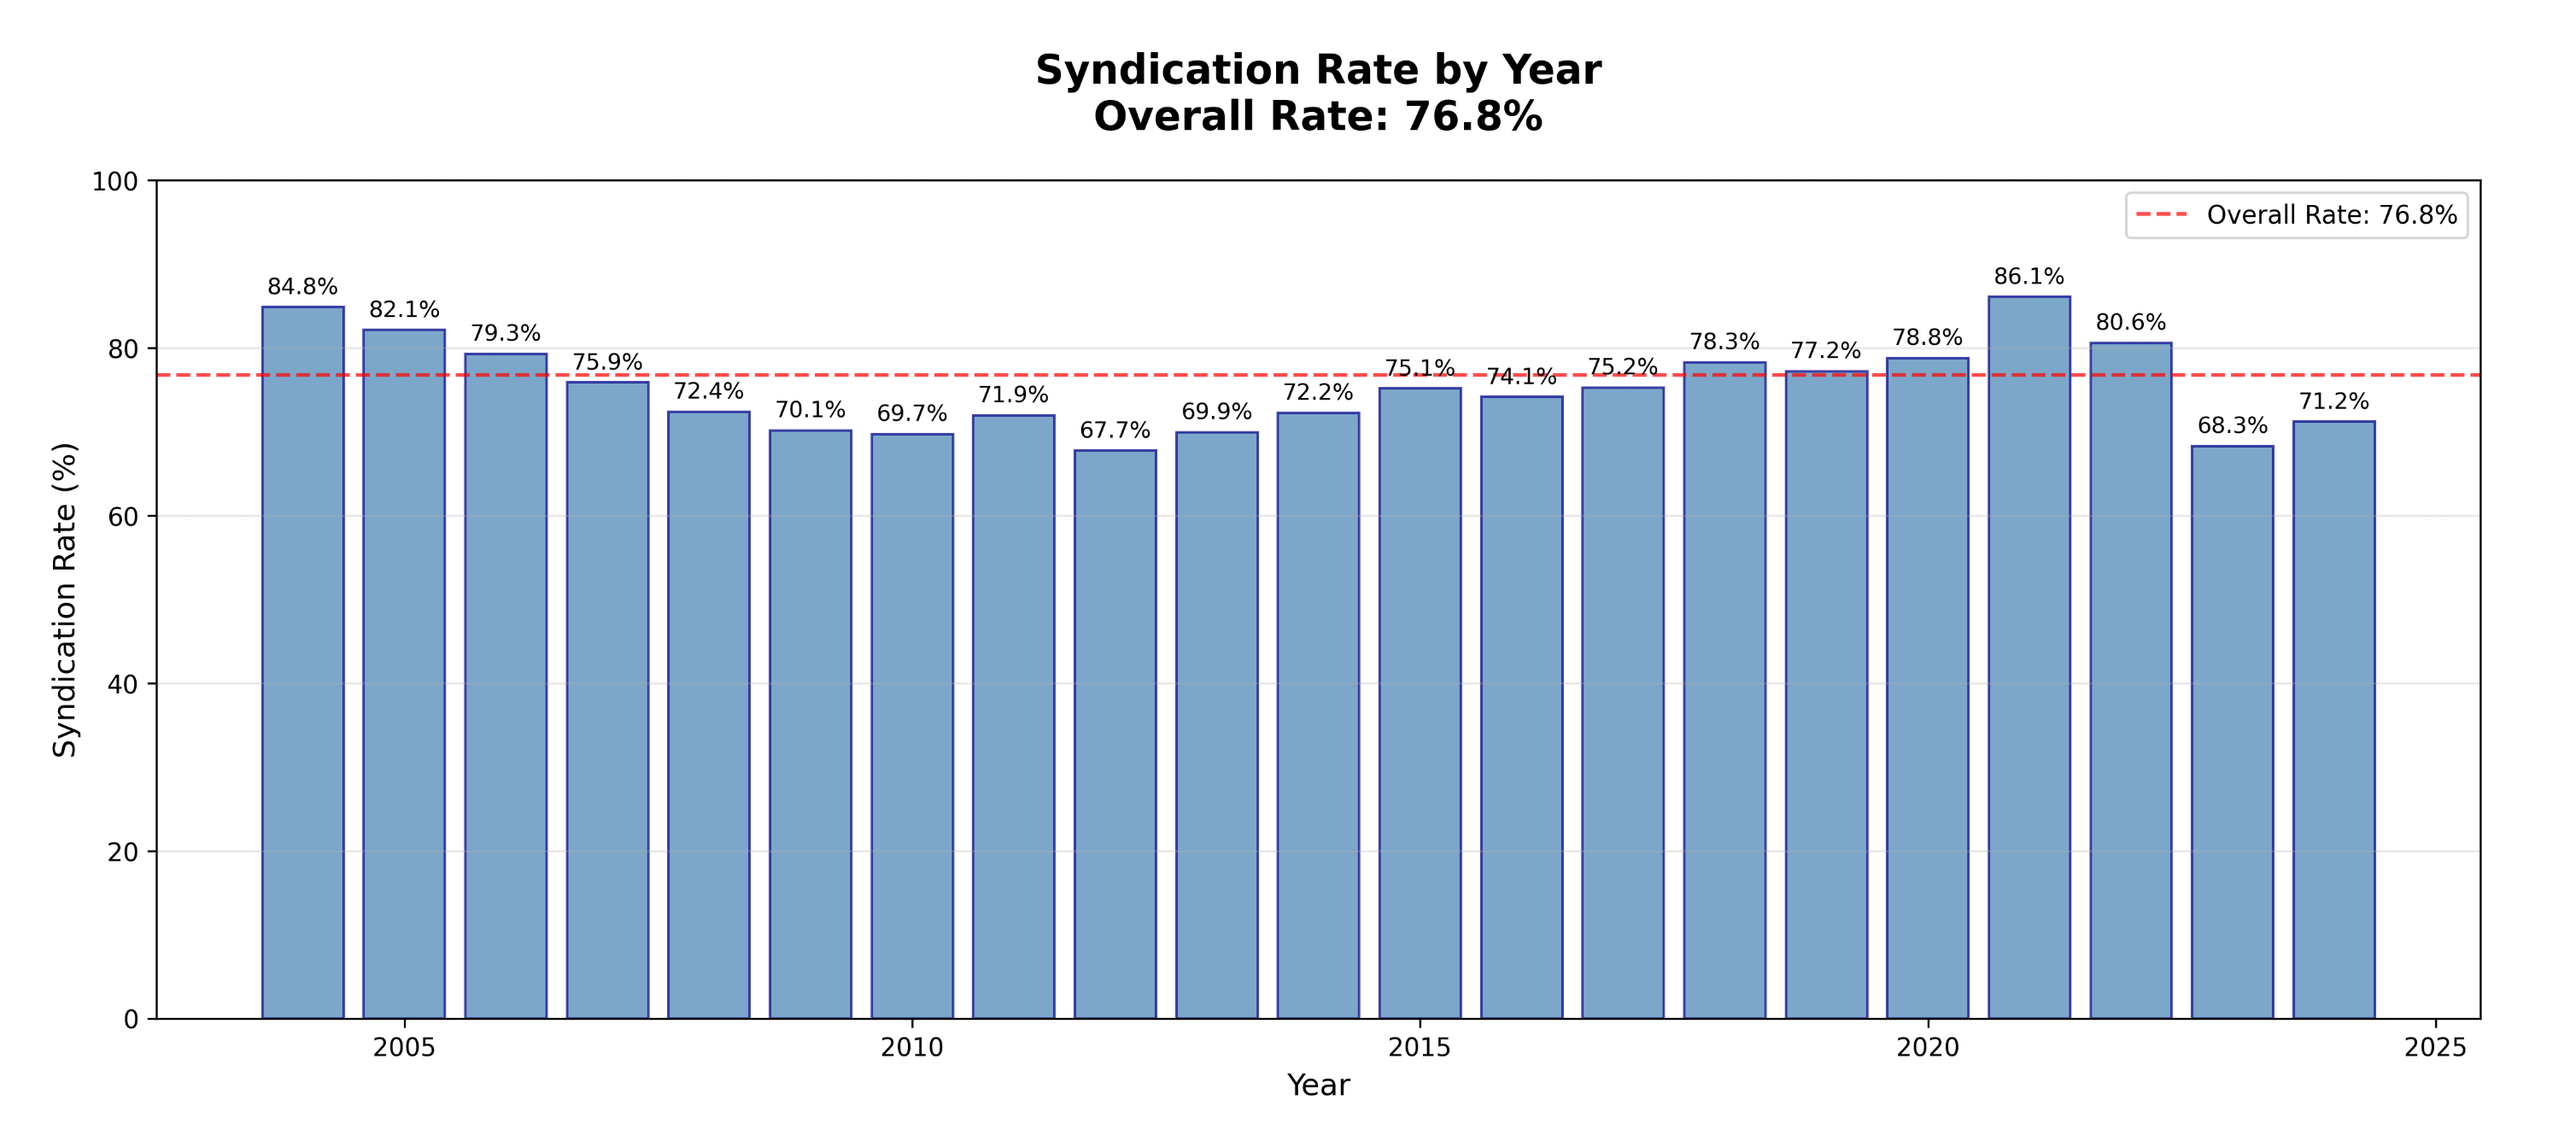
\includegraphics[width=0.8\textwidth]{../figures/mod/syndication_trends_v2.png}
    \caption{Syndication trends in US market}
\end{figure}
\vspace{1cm}
% \end{column}
% \end{columns}

\end{frame}

\begin{frame}
\frametitle{Research Gap \& Motivation}

\begin{block}{Current Limitation}
Traditional approaches models networks links regardless investor intrinsic characteristics.
\end{block}

\vspace{0.4cm}

\begin{alertblock}{Our Approach}
Apply Network Science theories to analyze coordination patterns in \textbf{early-late stage investor syndication networks} in the U.S. market.
\end{alertblock}

\vspace{0.3cm}

\begin{itemize}
    \item Broader understanding of systemic coordination patterns
    \item Need for \textbf{multidisciplinary perspective}:
    \begin{itemize}
        \item Finance \& Economic Sociology
        \item Network Science \& Ecology
    \end{itemize}
\end{itemize}

\end{frame}
